\documentclass[a4paper,12pt]{article} 
\usepackage[T2A]{fontenc}			
\usepackage[utf8]{inputenc}			
\usepackage[english,russian]{babel}	
\usepackage{amsmath,amsfonts,amssymb,amsthm,mathtools} 
\usepackage[colorlinks, linkcolor = blue]{hyperref}
\usepackage{upgreek}\usepackage[left=2cm,right=2cm,top=2cm,bottom=3cm,bindingoffset=0cm]{geometry}
\usepackage{graphicx}
\usepackage{multirow}
\usepackage{xcolor}
\author{Пазов Тенгиз}
\title{3.3.3. Опыт Милликена. Отчёт}
\date{16.09.2024}
\begin{document}
\maketitle
\newpage
\section{Цель работы} 
Измерение элементарного заряда методом масляных капель.
\section{В работе используются} 
Плоский конденсатор в защитном кожухе, измерительный микроскоп, электростатический вольтметр, электронный секундомер, переключатель напряжений, пульверизатор с маслом. 
\section*{Основные формулы}
Уравнение движения тела принимает вид:
\begin{equation}
m \dfrac{dv}{dt}=mg-F_{\text{тр}},
\end{equation}
где $m$ -- масса капли, $v$ -- её скорость, $F_{\text{тр}}=6\pi \eta rv = kv$ -- сила вязкого трения, $r$ -- радиус капли, $\eta$ -- коэффициент вязкости воздуха. Отсюда получаем 
\begin{equation}
v = \dfrac{mg}{k}\left(1 - e^{-kt/m}\right).
\end{equation}
\par Время релаксации тогда примет вид:
$$
\tau = \dfrac{m}{k}=\frac{v_{\text{уст}}}{g}$$
Обозначая $h$ путь капли, пройденный за $t_0$, получаем формулу для её радуса:
\begin{equation}
r = \sqrt{\dfrac{9\eta h}{2\rho gt_0}}.
\end{equation}

Новое слагаемое не влияет на $\tau$, новая установившаяся скорость
$$
v_{\text{уст}}'=\dfrac{qV/l - mg}{k}.
$$

\begin{center}
{$q = 9\pi \sqrt{\dfrac{2\eta^3 h^3}{g\rho}}\cdot \dfrac{l(t_0+t)}{Vt^{3/2}_0t}$}
\end{center}
\section*{Описание установки}
\begin{figure}[h]
    \centering
    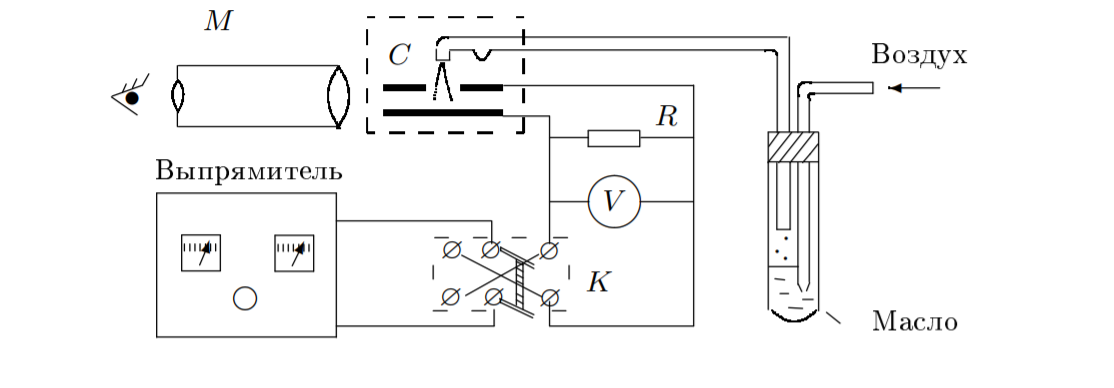
\includegraphics[scale=0.6]{1.png}
    \caption{Схема установки}
    \label{fig:your_label}
\end{figure}
Схема установки представлена на рис. 1. Масло разбрызгивается пульверизатором. Капли масла попадают в конденсатор C через неболь шое отверстие в верхней пластине. При этом часть из них вследствие трения о воздух приобретает случайный по абсолютной величине и зна ку электрический заряд. Напряжение на пластины подаётся от регулируемого выпрямителя и измеряется вольтметром V. Ключ К позволяет менять направление поля в конденсаторе, чтобы можно было работать как с отрицательно, так и с положительно заряженными каплями. При размыкании ключа К конденсатор разряжается через дополнительное сопротивление $R\approx10$ МОм.
\section*{Ход работы}

\par 1. Перед началом работы оценили с помощью формулы для нахождения заряда минимальное напряжение $U_{min}$, которое нужно для подъема капель, несущих 5 зарядов электрона на высоту h = 1 мм, задав $t \approx t' \approx 20 с$. Если в дальнейшем для подъема капель требовались меньшие напряжения, то соответствующие капли отсеивались нами, как непригодные для эксперимента. Расстояние между пластинами $l$ и плотность масла $\rho = 898$ $kg/sm^{3}$, коэффициент вязкости $\eta = 1,85\cdot10^{-5}$ $Pa\cdot s$(при температуре 300К).
\par 
	2. Включили осветитель. При этом направленный в камеру свет направлен под углом к оси микроскопа и в объектив не попадает. Поле зрения микроскопа поэтому остаётся тёмным. Капли масла рассеивают свет и выглядят светящимися точками на тёмном фоне. Не выключая электрическое поле, слегка надавили на грушу пульверизатора и наблюдали за движением облачка масляных капель в поле зрения микроскопа(изображение перевёрнуто).
	
\par 3. Настроили окуляр микроскопа на резкое изображение делений окулярной шкалы. Затем сфокусировали объектив на появившийся в рабочем пространстве капли.
\par 4. Наблюдая за движением капель, выбирали капли, время падения которых на $h = 1 мм$ лежит в пределах 10-30 с, и научились отличать их от более крупных, непригодных для работы.

\par 5. При начале опыта позволили капелькам свободно падать 5-10 с при выключенном электричческом поле для того, чтобы наиболее крупные капли упели упасть на нижнюю пластину. Из оставшихся в поле зрения капель выбирали по одной капле и производили с ней серию измерений, наблюдая ее падение под децствием силы тяжести и подъем под действием электрического поля.

\par 6. Проделали таких 5 измерений, каждый раз регистрируя величину U и получили график, на котором по оси отложены значения зарядов:
\begin{figure}[h!!]
    \centering
    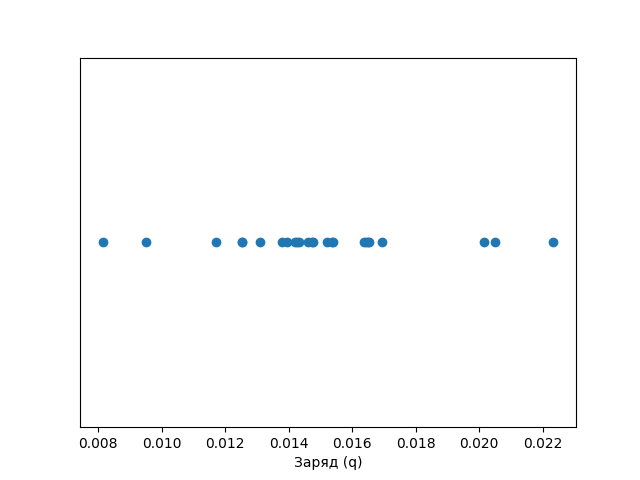
\includegraphics[scale=0.9]{my_graph.png}
    \caption{Заряды частиц, отложенные по оси Х}
    \label{fig:your_label}
\end{figure}
Как видно из данных значений в качестве элементарного заряда можно взять наименьший из перечисленных, то есть $q = 1.222 \cdot 10^{-19}$ Кл. Данная величина есть 76,27 \% от заряда, который обнаружил Милликен.
\section{Вывод}
В данной лабораторной работе измеряли элементарный заряд электрона, с помощью масляных капель, пульверизатора и конденсатора. Были получена пять средних значений для каждой из куч и выбрав самое маленькое значение пришли к выводу об элементраном заряде, равном $1.222 \cdot 10^{-19}$ Кл, что в система едениц СГС составляет $3.657 \cdot 10^{-19} СГС$, причем погрешность измерения данного элементарного заряда составила $\approx 0.15289 \cdot 10^{-19}$Кл как мы поймем из следующего файла. Данное значение составляет 76,27 \% от элементарного заряда, обнаруженного в 1910 году Милликеном. Как видно из файла с рассчетами погрешность измерения заряда составляет
\end{document}